%TC:ignore
\immediate\write18{texcount -inc -sum -utf8 main.tex > wordcount.txt}
%TC:ignore




\documentclass[12pt]{article}
\usepackage[margin=1in]{geometry}
\usepackage{natbib}
\usepackage{times}
\usepackage{hyperref}
\usepackage{setspace}
\doublespacing
\usepackage{booktabs}
\usepackage{threeparttable} 
\usepackage[table]{xcolor}
\usepackage{graphicx}
\usepackage{appendix}
\usepackage{siunitx}
\sisetup{round-mode=places, round-precision=3}
\title{Authoritarian IGOs and Constitutional Flexibility}
\author{Jihyeon Bae}
\date{}

\begin{document}

\maketitle

\begin{abstract}
Why would authoritarian states, often skeptical of legal constraints, adopt flexible amendment procedures for intergovernmental institutions that limit their own veto power? This article examines how the regime type composition of Intergovernmental Organizations (IGOs) shapes institutional rules for amending constitutive treaties. Using IGO-year panel data from 1960 to 2019, I show that IGOs dominated by authoritarian states are more likely to adopt majority-rule amendment procedures than their democratic counterparts. This counterintuitive pattern reveals that regime type shapes legal institutional design not only by influencing preferences for control, but also by altering the political costs of implementing collective legal change. These findings contribute to the intersection of constitutional flexibility, international legalization, and the strategic behavior of authoritarian regimes in global governance.
\end{abstract}

\section{Introduction}
How do member states design legal rules for constitutive amendments that underpin intergovernmental organizations (IGOs)—and how does regime type influence those design choices? While it is tempting to assume that autocracies prefer rigidity and control, this research note identifies a striking empirical pattern: authoritarian-dominated IGOs are more likely to adopt flexible amendment procedures, such as majority-rule voting without ratification requirement, that reduce individual member states’ ability to block unwanted amendments to constitutive treaties.

Intuitively, one might expect authoritarian states and their own IGOs to hold onto veto powers in order to shield themselves from unwanted treaty amendments—especially when democracy-led IGOs are perceived as externally constraining. Yet recent research on authoritarian international cooperation suggests that autocratic states are increasingly building their own formal institutions, coupled with codified treaties and bureaucratic organizations that can reinforce regime durability and reduce democratization risks (\cite{debre2021}).

Once we begin to take international law as a tool actively shaped and managed by authoritarian states, important variation in institutional design comes into view. I argue that, contrary to conventional wisdom, authoritarian-dominated IGOs are more likely than democracy-led IGOs to adopt flexible amendment rules that reduce individual member control over treaty change.

When authoritarian states predominantly hold seats at IGOs, authoritarian states are actually better positioned to give up veto power on amendments for IGOs’ constitutive treaties. This is due to two factors. First, even when authoritarian states end up having to accommodate less desirable amendments, they can soften the blow by framing the issue to be less salient. Plus, it is expected that the deviation between amendment choices from the rest of the group and individual country will be minimal, since authoritarian IGOs tend to be homogeneous in terms of cautionary actions against potential democratization risk factors.  

This paper contributes to the current understanding of the relationship between regime type and constitutional control in several ways. First, it bridges the literature on domestic constitutional design with theories of institutional design in intergovernmental organizations (IGOs). While scholarship on IGOs has largely focused on unequal control over agendas through mechanisms like weighted voting ({Koremenos et al., 2003}), much less attention has been paid to how all member states—regardless of power differentials—jointly determine the level of control over constitutional amendments. 

Meanwhile, comparative constitutional law has developed rich theories explaining amendment frequency and rigidity in domestic systems, but these insights have rarely been applied to the constitutive treaties of international organizations. For example, Ginsburg has tackled the methodological challenge of measuring constitutional flexibility, with an emphasis on an amendment culture (\cite{ginsburg2015}). 

Similar to arguments from the international institutions scholarship, amendment difficulty is understood to increase as voting thresholds become higher (\cite{lutz1994, ferejohn1997}). While there is meaningful overlap over the study of constitutional flexibility in realms of domestic politics and IGOs, there have been limited studies on the latter.  The concept of constitutional control, understood as the collective willingness of states to make joint decisions on treaty revision, has not been treated as a central element of design at the IGO level compared to domestic judicial studies. This paper expands the concept of constitutional amendment from the domestic to the international level, offering a novel framework for understanding how regime type shapes the flexibility of global governance structures.  

Second, I show that authoritarian states can opt for an institutional design choice that requires sacrifice in domestic policy autonomy. Rather than uniformly rejecting any risk of facing sub-optimal collective amendment, the circumstances favorable to majority rule incentivizes authoritarian states to give up veto power on amendments more so than democracies. By showing authoritarian states’ willingness to loosen control over IGO’s rule, I add complications to the conventional wisdom that countries of weak domestic rule of law would refrain from making commitment to inter-governmental institutions. 

Last, I bring an interesting insight that institutional design choices can lie not just on the “pull” factor around the benefits, but also the cost of implementing certain features. Even when all regime types can greatly benefit from the simple majority rule that grants flexibility in the era of uncertainty, only some states can afford to give up their veto power. I emphasize the importance of considering the domestic political cost, procedures of implementing and justifying unwanted collective decisions on amendment. 

\section{Authoritarianism and International Law}
In this section, I situate the theme of authoritarian states’ cooperation through formal Intergovernmental Organizations (IGOs) along with codified constitutive treaties. To paint a clearer picture of what these clubs of authoritarian states look like, I include an illustrative case of Myanmar showing how the ASEAN (Association of Southeast Asian Nations) Charter was invoked. The former Myanmar’s leader, Aung San Suu Kyi invoked the principle of non-interference in her favor amidst charges of genocide committed against the Rohingya Muslim minority. During the UN Security Council meeting, Myanmar expressed its gratitude toward members of the Security Council “who upheld the principle of non-interference in the internal affairs of sovereign countries,” and condemned  liberal democracies’ pressure as an act of infringement on sovereignty.  When the topic of junta was broached, members of ASEAN invoked the principle of non-interference in the Charter  and maintained a rather acquiescence stance, by calling the coup “an internal affair” that remains in Myanmar. 
It is not just an anecdotal case that intergovernmental projects with like-minded autocrats indeed directly help regime survival against democratization pressure. Recent literature on authoritarian international law has highlighted how autocracies are not merely passive recipients of international norms but are actively shaping legal frameworks to reflect their interests (Ginsburg, 2020). In Debre’s (2021) seminal work, authoritarian state leaders who have been members of authoritarian clubs tended to survive longer in their incumbencies, everything else equal. IGOs as focal points help authoritarian leaders maintain incumbency through learning and coordinating (Hall and Ambrosio, 2017; Bank, 2017; von Soest, 2015; Obydenkova \& Libman, 2019). In this sense, Authoritarian IGOs and their constitutive treaties that enshrine the key principles of authoritarian cooperation are crucial tools for authoritarian survival, rendering further gravity to the topic of how these treaties are amended.
According to Hooghe et al. (2017), the constitution of an IGO refers to “a set of fundamental principles or established precedents for the governance of an organization.” For consistency, I use the term “constitution” to denote the organization’s supreme law that publicly declares its foundational principles and goals. IGO constitutions take various names and forms. For example, some organizations are established through documents labeled “Constitutive Instruments,” “Treaty,” or “Charter” (Hooghe et al., 2015). Regardless of terminology, the supreme law at the apex of an organization’s legal framework is typically a constitutive treaty adopted at the IGO’s inception. To clarify the paper’s central focus, I examine whether IGOs composed of autocratic states adopt more relaxed rules for proposing and enforcing amendments to their constitutions.

\section{Constitutional Control and Institutional Design}

I define “constitutional control” as the degree to which IGO member states collectively shape and constrain constitutional amendment processes. This includes both the voting threshold required to adopt an amendment and the domestic ratification requirements for implementation. An IGO where members have strong constitutional control would expect a rigid constitution, as it requires more members’ agreement and persuasion to adopt and also implement the amendment. On the other hand, an IGO with members having weak constitutional control would anticipate a more flexible constitution. Voting rule and the requirement for the implementation of the voting result are the two most prominent and observable aspects of constitutional control. 

There are several factors that motivate states to opt for unanimity rule, increasing the overall state control over constitutional changes. States are incentivized to preserve their individual veto power when they are uncertain about how the cooperation would look in the future (Koremenos et al., 2000). For example, when IGOs cover issue areas that are prone to technical advancement, it poses a high level of uncertainty about who will gain or lose more from cooperation. In such cases, states tend to prefer keeping veto power for amendments so that they can have a final say in collective decision making. 

\subsection{Regime Type as an explanatory variable}

So far, I have reviewed existing explanations on varying constitutional control over amendments. Both rational design of institution literature and domestic constitution theory emphasize benefits of voting rule options to explain design outcomes ex post. The logic states that if states have much to gain by making it easier for all states to amend the constitution, then they favor simple majority rule instead of unanimity. When individual member states have full control over amendments of the collective constitution, it adds more hurdles for changes. While the “pull” side of the story emphasizes potential gains from constitutional control options, I show that the “push” side of calculation matters too.
I propose regime types of member states of an IGO as the key explanatory factor for constitutional control. Regime type adds a unique analytical benefit since the degree of uncertainty varies similarly across different types of domestic political structures. Hence, addition of regime type can contribute to explaining the remaining variation in constitutional control after taking uncertainty into account. I argue when states decide on institutional design choices, their cost is related to regime types and associated domestic political structures. 

\subsection{Domestic Political Cost of Majority Rule}

Relative to unanimity rule, majority rule can allow for a lower threshold to influence a collective decision (Posner and Sykes, 2014). While majority rule allows room for flexibility, states have to give up veto power and forgo individual control over constitutional changes (Buchanan and Tullock, 1965). This comes at the risk of subsuming to unwanted decisions on constitutional amendment reached by the 51\% of the group whereas the country is on the other 49\%. On the other hand, while unanimity rule allows full control over amendment, it incurs negotiation costs on all parties until they reach a consensus. Benefits of majority rule versus unanimity rule are clear. What remains underexplored is the political cost of each decision rule around amendments. 
IGOs composed of authoritarian states are better positioned to accept the cost of being on the 49 \% on amendment. This is because the cost of adjusting domestic policies in order to comply with the collective decision is lower for authoritarian state leaders. My argument emphasizes costs attached with constitutional control, as I look at not only what states want and how they benefit, but also what is an available option for different domestic political circumstances.

With Buchanan and Tullock’s model on decision making rules (1965), the closer a voting rule is to unanimity, the higher the external cost is. External cost is incurred when a participant is forced to follow the collective decision that is deviant from one’s own preference. When member states adopt an amendment for an IGO’s written rules that they otherwise would not have supported, external cost gets higher. In other words, it is determined by the expected cost of having to adhere to collective decisions and readjust domestic policies accordingly.

I further break it down into two components that align with states’ institutional design choices: (1) expected distance between potential unwanted result and each member’s own preference point and (2) significance of adopting an unwanted decision.  

In the next section, I use this framework to expand the argument that regime type shapes the cost function around various voting rules. First element of external cost is the expected readjustment cost (both political and fiscal) of making domestic changes for a new amendment. States have to explain and justify why such a new direction is wanted and adjust domestic rules in ways that align with collective interests by setting up relevant bureaus. Authoritarian state leaders have greater leeway in both aspects. 

Constitutional amendments bring about significant political ramifications on the ground. The ASEAN Charter, for example, has gone through multiple amendments, as collective gains to harvest were large and it provided enough incentives for members to invest resources to make amendments. Several amendments for the ASEAN Charter added more specific action plans like implementing the shared database of non-tariff measures, and accelerating free trade by removing non-traditional barriers (ASEAN Framework (Amendment) Agreement for the Integration of Priority Sectors, November 2004). Some of the changes require a substantial amount of domestic effort, given the level of precision. Member states were expected to pay the economic cost of implementing new administrative task forces and the political cost of legitimating changes and appropriation of budget. The argument I’m making here is that these readjustment costs are significantly lower for authoritarian states than democracies. 

To illustrate a short example of Thailand, one of the key members of the ASEAN, Prime Minister Yingluck Shinawatra during the administration in 2014 had to answer the question regarding amendments raised by a competing party leader about whether the country is prepared to manage free movement of laborers from ASEAN community given its dependence on agricultural and labor-intensive industries. The question was raised with a reference to the ASEAN Framework Agreement that specified a 5-year plan. There were several parliamentary debates before and after the ASEAN meeting, given the cost of political adjustments even for authoritarian states. But the degree to which such a political cost hampers state leaders’ approval rate (from either constituents or internal factions) is significantly low for  authoritarian states. 

For sharp comparison, liberal democracies as respondent governments use international organizations as a scapegoat when incumbents need to appease constituents, especially when the dispute has high political salience (Lim and Lee, 2022). Dai (2007) further suggests that liberal democracies align themselves with key interest groups and decide compliance behavior. Indeed, policies around engagement with international organizations are alarmingly becoming key polarization forces in democracies. Of course, both regime types do have to explain policy adjustments, but the magnitude of failure to do so is different. 

Second component of external cost is the expected distance between each authoritarian state’s ideal policy point and deviating collective decision. The distance between the new constitution’s pursuit and each member state’s ideal point is expected to be small for a group of authoritarian states, as they prioritize principle of non-intervention over other competing values. Changing an IGO’s constitution in ways that introduce risk factors that might menace one authoritarian regime survival means a threat to all given cascade effects of democratization. With a shared fate and homogeneous priority, authoritarian states’ do not expect the worst-case scenario of having an entirely new normative goal. Politicians and their parties in liberal democracies directly pay for the cost of implementing collective decisions that deviate from the constituents’ preferences. 

In sum, authoritarian states are in a better position to opt for majority decision rule compared to democratic states. They are more likely to embed individual decisions together as a group, owing to readiness to accept sub-ideal decisions around constitutional reform. 
Hypothesis: The higher an IGO’s average autocracy score, the closer its voting rule for constitutional reform is to majority rule.

\begin{itemize}
  \item \textbf{Hypothesis:} \textit{The higher an IGO’s average autocracy score, the closer its voting rule for constitutional reform is to majority rule.}


\section{Data and Methods}
The following sections provide empirical strategies to test the theoretical expectation outlined above. I use panel data of 73 IGOs from 1960 to 2019 traced by the “Measuring International Authority (MIA)” (Hooghe et al., 2017). This time scope well captures the landscape of international governance at the beginning of the second democratization wave and in a less ideology-driven setting (Strand et al., 2012). To measure the level of democracy for members, I use the polyarchy score, ranging from 0 to 1 from the Varieties of Democracy project (Coppedge et al., 2017). I merge the MIA dataset with Correlates of War data (2019) which focuses on formal organizations to get general information about the organization, including whether it’s designed to tackle general or task-specific goals. This excludes ad hoc groups that are designed to serve a short-term goal like the Cairns group and informal groups lacking independent secretariat like G8.


\subsection{Constitutional control and pooling}

To operationalize the concept of constitutional control, I use the “constitutional pooling” variable from the MIA dataset, which captures the extent of joint decision-making authority over amendments, incorporating both voting rules and ratification constraints. While constitutional control is a broader concept that includes states’ capacity to shape, block, or implement treaty amendments, the “constitutional pooling” measure from the MIA project offers the most systematic proxy focusing on observable implications. It captures key features such as voting rules and ratification requirements that reflect the degree of collective constraint on constitutional change. Although it cannot capture informal mechanisms or enforcement dynamics, it provides a reliable cross-IGO comparison over time.

\begin{table}[ht]
\centering
\rowcolors{2}{gray!15}{white}
\begin{tabular}{>{\bfseries}l l >{\bfseries}l p{7cm}}
\toprule\multicolumn{2}{c}{\textbf{Voting Rule}} & \multicolumn{2}{c}{\textbf{Ratification Requirement}} \\
\midrule
0     & Individual members decide             & 0.25  & Ratification required by all \\
0.33  & Unanimity                             & 0.50  & Ratification required by a subset, result binding on subset \\
0.66  & Supermajority                         & 0.75  & Ratification required by a subset, result binding on all \\
1     & Simple majority                       & 1.00  & No ratification required \\
\bottomrule
\end{tabular}
\caption{\textbf{Two Components of Pooling on Constitutional Reform}}
\label{fig:pooling-components}
\end{table}

What does it look like for an IGO to completely pool decision making power around constitutional revision? Under this scenario, member states forgo veto power and lower the bar for passing amendments to simple majority. Yet, pooling means something more than a simple voting rule. One important factor of decision making in the international realm is that the decision outcome possesses little to limited power if every member’s ratification at domestic level is required for the amendment to come into effect. The ratification clause requires that international decisions be domestically approved in member states’ legislation. It can practically nullify a new amendment that has been approved with unanimity rule. Existence of ratification requirement thus decreases pooling score, even when the group chooses majority voting rule. 

Pooling score on constitutional reform increases as a decision rule for amendment gets closer to majority rule, further from unanimity rule. Simple majority decision rule gets a higher pooling score than two thirds, and unanimity rule (consensus). In addition, the more ratifications an IGO needs to fully implement the amendment, the less score it gets on pooling. The Gulf Cooperation Council, for example, employs the unanimity rule for new amendments to the Charter of the Gulf Cooperation Council.  Although the GCC requires unanimity, ratification isn’t required and once the amendment passes, it’s automatically in action. In the case of the League of Arab States, even though two thirds majority voting rule is employed for constitutional amendments, ratification is required which gives way more latitude for members to opt out by not ratifying it. Pooling score is an inversely weighted voting rule with respect to ratification requirements.

\subsection{Measuring democracy at the IGO level}
I use an average score of V-Dem’s “polyarchy” among member states, which shows the average level of electoral democracy in one IGO. Conventionally, regimes with scores of 0.5 and above are considered democracies. To measure the level of democracy of an IGO, instead of a single country, I constructed the IGO-level democracy score by formulating the average polyarchy score of all the member states in each IGO. 

\textbf{\textit{Political and preference heterogeneity among members}}

I measured member states' heterogeneity in terms of their regime types by using standard deviation of members' V-Dem polyarchy score from the mean of an IGO. This proxies a distribution of political disparity among member states at an IGO level. International organizations scholarship (Obydenkova 
$&$Libman, 2019) show that AIGOs tend to have homogenous membership composition. Mansfield and Pevehouse (2006) shows that democracies prefer having similar democracies as new members of their international organizations. This is attributed to the pattern that DIGOs include economic or human rights conditions upon a new member’s accession, while AIGOs do not. Heterogeneity is expected to affect both IGO’s average democracy score as well as constitutional pooling.

To directly operationalize observable heterogeneity seen among one another, I created another variable preference heterogeneity that is based on standard deviation of “state ideal points” from the United Nations General Assembly voting results (Bailey et al., 2017; Voeten, 2000). Since voting results are publicly available to state representatives, this variable offers a good way of measuring “perceived” compatibility in policy directions and preferences among member states. \cite{bailey_estimating_2017} estimated ideal points using the UNGA voting data that are comparable across time and issue areas. 

\textit{Economic Factors}

If members are heavily reliant on international trade, then an IGO is expected to have a higher level of pooling as domestic interest groups ask for more cohesive cooperation across the borders to facilitate trade. Trade variable is an average score of total trade volume including exports and imports, from the World Bank’s World Development Indicator. Note that this variable is about member states’ overall exposure to trade with any external actors, not limited to trade partners amongst themselves. Logged GDP per capita is a simple average of members’ GDP per capita (in constant 2015 US dollar values) from the World Bank’s Development Indicator. It can be contended that members’ economic developments ultimately determine institutional designs. Without cooperation among authoritarian states, authoritarian leaders themselves can single-handedly manage democratization pressure due to affordability of better military logistics. Population is another indicator of power-based explanation along with GDP per capita and Trade variables. 

\textit{Number}

Having too many states with a distinct set of preferences is considered as a major obstacle for an integration. Institutions can produce collective goods when they make members easier to punish cheaters and reduce transaction costs. To overcome the problem of large N, states often resort to creation of international organizations (Guzman, 2008; Abbott \& Snidal, 1998). In this regard, levels of pooling are expected to increase with the size of an organization. 
Alliances

If an IGO is composed of members who have many allies around the world, relative value of having a tie with an IGO will be meager compared to a group of pariah states who have no other states to rely on. If a pursuit of logistical support or material needs were the main motivations for regional integration with legal components, we would observe an IGO whose members are not popular allies to have higher levels of pooling. I use each members’ number of alliances from the Alliance Treaty Obligations and Provisions (ATOP) dataset (Leeds, 2005). 

\textit{Economic and Political disparity (HHI)}

If members’ economic disparity is large within one IGO, members will want to reserve their own veto power so that rich states’ interests don’t subsume weak states’ preferences. Allee et al. (2016) posits that preferential trade agreements that involve states with significant power imbalance tend to have strong dispute settlement mechanisms. 

For example, if weak states fear strong states’ potential amendments that call for further resource contributions to an IGO, having a voting rule that is close to unanimity can be helpful. If the economic disparity were large, we would expect a low level of pooling since weaker states might empower the secretariat to have strong states share power with an independent organization’s bureaucracy. Functionally, I use the Herfindahl-Hirschman (HH) index. While it is often used to measure market asymmetry, it can be applied to international institutions in a way of operationalizing to what extent a few members are dominating the group in terms of economic sizes (Smith, 2000).  

\textit{Political, Social and Economic}


IGOs serve various purposes, handling functional goals of environmental or economic agendas and political goals. The binary variables, social and economic, indicate the primary purposes of an IGO based on their initial contracts. Initial dataset from the COW project includes the third category, political, which is the baseline for the comparison. This tests whether IGOs that address task-specific goals are more likely to push for legalization based on various interest groups compared to those that serve general political agenda. Organizations that were designed to be political arena are expected to have lower pooling scores given the sensitivity of political questions compared to social and economic tasks. 

\textit{Colonial Legacy}

Experience of colonialism and its institutional impacts can be a potential confounder between the relationship between regime types and a collective voting rule. Postcolonial countries, often experiencing weak domestic legal institutions, are less favorable to the right of veto which empowers a single country over the majority preference. Authoritarian states’ preference for majority rule might not be the effect of their domestic politics, but instead, historical legacy as a confounder.

\subsection{Estimation Strategies}

To test whether there is a positive correlation between the level of democracy for an IGO and degree of pooling on constitutional reform decisions, I use different estimation strategies that minimize the sensitivity of results from statistical models. Construction of a year-fixed effect estimator removes year specific shocks that could influence an IGO’s constitutional pooling. I use heteroskedasticity-consistent standard errors for all models.  Panel heteroskedasticity arises when different units have different variances. The variance of pooling score is expected to be different across IGOs since there is a greater heterogeneity for economic sizes for authoritarian IGOs. Hence, it is both theoretically and methodologically crucial to adjust for a heteroskedasticity problem. This puts my hypotheses under much more conservative tests in terms of statistical significance. The results are consistent, in terms of variables that are statistically significant as well as the direction of correlation.  


\section{Empirical results and discussion}

Using the panel data with the unit of analysis at IGO-year, I ran regression models on the main dependent variable, “constitutional pooling” High pooling score indicates a strong collective willingness in a form of giving up their veto power on new amendments. Across all models and measurements of democracy, there have been consistent positive relationships between an IGO’s level of  authoritarian states and constitutional pooling. The more authoritarian states there are in an IGO, the more likely they are to move towards majority rule instead of unanimity rule for introducing and adopting amendments for their IGO-level constitution. 

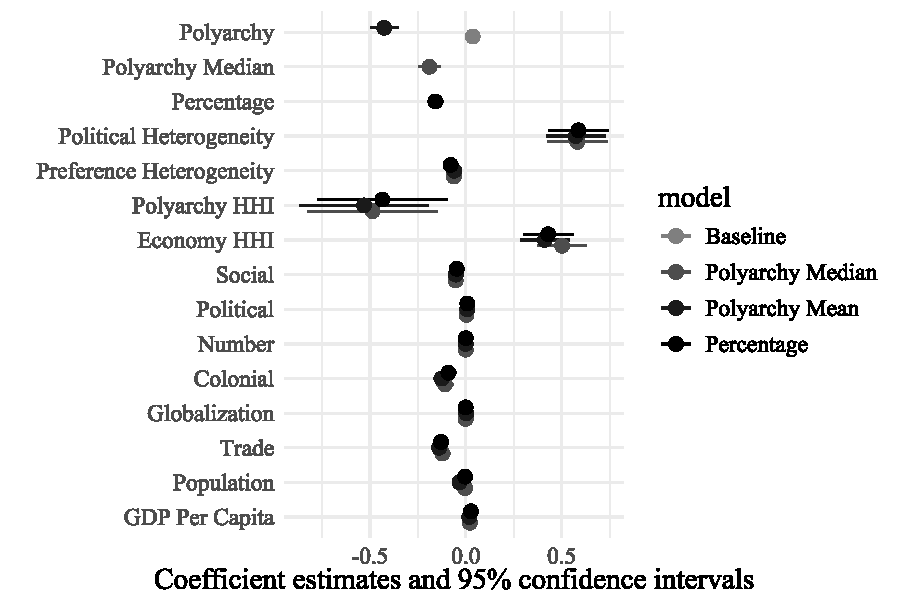
\includegraphics{amendment_aigo/pooling_result.pdf}

Figure 2 shows estimated coefficients between average polyarchy score and pooling for constitutional reform. Line around the point estimates shows a 95\% confidence interval around the estimate. Variable polyarchy showed negative coefficients with statistical significance even after considering a battery of control variables. Substantively, a one-point drop in polyarchy (from full democracy to full autocracy) is associated with a 0.658-point increase in pooling—equivalent to the change in voting rule from unanimity to simple majority.

This effect is even larger than the shift introduced by changing ratification requirements (e.g., from no ratification required to requiring approval by a subset of members). These results hold after controlling for time-fixed effects and other confounding variables, suggesting that authoritarian IGOs—due to both greater gains from procedural flexibility and lower domestic political costs—are more inclined to adopt majority-based rules for constitutional control.



Auxiliary variables show mixed results. Specifically, the greater the average number of alliances that members of an IGO had, the lower the pooling score on constitutional reform is. This suggests that alternative avenues of support from allies diminish the enticement of cooperation gains derived from maintaining flexibility within the IGO. 

Additionally, it is proposed that alliance complexity increases the stakes of institutional decisions, thereby making veto power more desirable. The larger the size of an IGO is, the less likely it is to have strong pooling around constitutional reform. This is contrary to what has been suggested in existing literature (Koremenos et al., 2001; Oye 1986). I suggest it might be attributable to the idea that states might expect greater external cost when there are more actors involved around the issue area and choose to minimize the sovereignty cost. On average, an IGO with a political task is expected to have a higher pooling score compared to those with social and economic goals. An IGO with economic goals would contribute to policy-oriented cooperation, which can be translated into domestic policy adjustments more easily than IGOs with broad political and social tasks. In the same logic as I have described, an IGO given with a political goal can enjoy lower external cost. Logged GDP per capita, population, and trade volume had a mixed result, rendering weak support for realist claims. Despite the concern around the confounding effect of a country’s colonial history, whether an IGO was largely composed of post-colonial states did not have any statistically significant impact on the output variable. Similarly, distribution of economic sizes and regime type heterogeneity did not show any meaningful results. 


\section{Conclusion}
This research note addresses an important puzzle for both legal scholars and political scientists: Why would authoritarian governments—often seen as defenders of sovereignty and opponents of international legal constraint—voluntarily give up veto power over constitutional amendments? This is an underexplored intersection of international law, institutional design, and authoritarian politics. While conventional wisdom suggests that authoritarian states would cling to unanimity rules to preserve control, this study finds that autocracies—when cooperating with like-minded regimes—are more likely to adopt majority-rule frameworks. This counterintuitive finding highlights how lower external political costs and shared regime interests allow authoritarian states to prioritize flexibility over control. These results challenge assumptions about authoritarian resistance to legal commitment and extend theories of constitutional design into the international arena. Future research could supplement these findings with case studies to further unpack the political calculations behind authoritarian cooperation in IGO governance.
\bibliographystyle{plainnat}
\bibliography{refs}


\begin{appendices}
\section{Regression Tables}

\input{amendment_aigo/pooling_table_clean.tex}

\end{appendices}

\end{document}
